\section{Kiểm thử và đánh giá hệ thống}
\label{chap:kiemthu}

\begin{indentParagraph}
Chương này trình bày quá trình kiểm thử và đánh giá hệ thống truy xuất thông tin đa phương thức từ âm thanh. Nội dung bao gồm chiến lược kiểm thử, các độ đo đánh giá, kết quả thực nghiệm, phân tích sai số, và đối chiếu với yêu cầu đặt ra.
\end{indentParagraph}

\subsection{Chiến lược kiểm thử}

Hệ thống được kiểm thử theo ba cấp độ từ thấp đến cao để đảm bảo chất lượng toàn diện. Ở cấp độ thấp nhất, Unit Tests kiểm thử từng module riêng lẻ bao gồm ASR, Chunking, Embedding và RAG để đảm bảo mỗi thành phần hoạt động đúng theo đặc tả. Cấp độ tiếp theo là Integration Tests kiểm thử khả năng tích hợp và giao tiếp giữa các module, phát hiện các vấn đề về interface và data flow giữa các thành phần. Ở cấp độ cao nhất, End-to-End Tests kiểm thử toàn bộ pipeline từ input đến output, mô phỏng các tình huống sử dụng thực tế của người dùng.

\begin{table}[H]
    \centering
    \caption{Công cụ kiểm thử sử dụng}
    \label{tab:test_tools}
    \begin{tabular}{|l|l|p{6cm}|}
        \hline
        \textbf{Công cụ} & \textbf{Mục đích} & \textbf{Mô tả} \\
        \hline
        pytest & Unit/Integration testing & Framework kiểm thử Python phổ biến \\
        pytest-cov & Code coverage & Đo độ phủ mã nguồn \\
        unittest.mock & Mocking & Giả lập các dependencies \\
        \hline
    \end{tabular}
\end{table}

\subsection{Các module được kiểm thử}

\subsubsection{Module ASR}
Kiểm thử khả năng transcribe audio với các test cases bao gồm transcribe audio ngắn (dưới 1 phút), kiểm tra độ chính xác của word-level timestamps, tích hợp VAD lọc đoạn im lặng, và xử lý audio dài (trên 30 phút).

\subsubsection{Module Chunking}
Kiểm thử các phương pháp chia nhỏ văn bản bao gồm fixed-size chunking với overlap, semantic chunking giữ nguyên ngữ nghĩa, và bảo toàn timestamps cho audio chunks.

\subsubsection{Module Anti-Hallucination}
Kiểm thử cơ chế chống ảo giác bao gồm phát hiện câu trả lời fully grounded, phát hiện câu trả lời hallucinated, phát hiện conflict giữa các nguồn, và safe abstention cho câu hỏi ngoài phạm vi.

\subsection{Độ đo đánh giá}

\subsubsection{Độ đo cho Information Retrieval}

Các độ đo tiêu chuẩn trong Information Retrieval được sử dụng \cite{manning2008ir}:

\textbf{Mean Reciprocal Rank (MRR)} \cite{voorhees2000mrr}: Đo vị trí trung bình của kết quả đúng đầu tiên:

\begin{equation}
    MRR = \frac{1}{|Q|} \sum_{i=1}^{|Q|} \frac{1}{rank_i}
    \label{eq:mrr_eval}
\end{equation}

\textbf{Normalized Discounted Cumulative Gain (NDCG)} \cite{jarvelin2002ndcg}: Đánh giá chất lượng xếp hạng có trọng số.

\textbf{Recall@K}: Tỷ lệ tài liệu liên quan được tìm thấy trong top-K kết quả.

\subsubsection{Độ đo cho Question Answering}

\textbf{Grounding Accuracy}: Tỷ lệ câu trả lời được xác minh từ nguồn.

\textbf{Abstention Rate}: Tỷ lệ từ chối trả lời đúng khi không đủ thông tin.

\subsection{Bộ dữ liệu đánh giá}

\begin{table}[H]
    \centering
    \caption{Bộ dữ liệu đánh giá}
    \label{tab:eval_dataset}
    \begin{tabular}{|l|c|c|}
        \hline
        \textbf{Loại dữ liệu} & \textbf{Số lượng} & \textbf{Mô tả} \\
        \hline
        Audio files & 50 & Bài giảng, thông báo (tiếng Việt) \\
        PDF documents & 80 & Quy định, biểu mẫu \\
        Tổng chunks & 3,420 & Sau khi chunking \\
        Test queries & 100 & Câu hỏi đánh giá \\
        Ground truth & 100 & Câu trả lời chuẩn \\
        \hline
    \end{tabular}
\end{table}

\subsection{Kết quả thực nghiệm}

\subsubsection{Kết quả Retrieval}

\begin{table}[H]
    \centering
    \caption{Kết quả đánh giá Retrieval}
    \label{tab:retrieval_results}
    \begin{tabular}{|l|c|c|c|c|}
        \hline
        \textbf{Phương pháp} & \textbf{MRR} & \textbf{NDCG@5} & \textbf{Recall@5} & \textbf{Recall@10} \\
        \hline
        Vector only (SBERT) & 0.62 & 0.58 & 0.68 & 0.75 \\
        BM25 only & 0.55 & 0.51 & 0.62 & 0.70 \\
        Hybrid (RRF) & 0.70 & 0.66 & 0.75 & 0.80 \\
        Hybrid + Rerank & \textbf{0.75} & \textbf{0.71} & \textbf{0.78} & \textbf{0.83} \\
        \hline
    \end{tabular}
\end{table}

Hình \ref{fig:retrieval_chart} minh họa trực quan sự cải thiện của các phương pháp retrieval:

\begin{figure}[H]
    \centering
    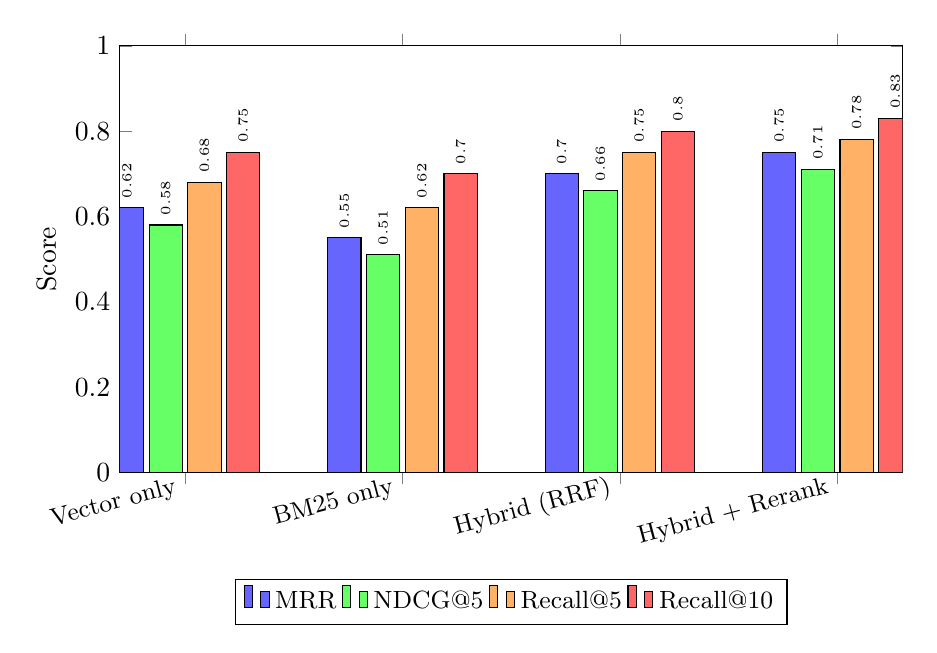
\begin{tikzpicture}
        \begin{axis}[
            ybar,
            bar width=12pt,
            width=0.95\textwidth,
            height=7cm,
            ylabel={Score},
            symbolic x coords={Vector only, BM25 only, Hybrid (RRF), Hybrid + Rerank},
            xtick=data,
            x tick label style={rotate=15, anchor=east, font=\small},
            ymin=0, ymax=1,
            legend style={at={(0.5,-0.25)}, anchor=north, legend columns=4, font=\small},
            nodes near coords,
            nodes near coords style={font=\tiny},
            every node near coord/.append style={rotate=90, anchor=west},
        ]
            \addplot[fill=blue!60] coordinates {(Vector only,0.62) (BM25 only,0.55) (Hybrid (RRF),0.70) (Hybrid + Rerank,0.75)};
            \addplot[fill=green!60] coordinates {(Vector only,0.58) (BM25 only,0.51) (Hybrid (RRF),0.66) (Hybrid + Rerank,0.71)};
            \addplot[fill=orange!60] coordinates {(Vector only,0.68) (BM25 only,0.62) (Hybrid (RRF),0.75) (Hybrid + Rerank,0.78)};
            \addplot[fill=red!60] coordinates {(Vector only,0.75) (BM25 only,0.70) (Hybrid (RRF),0.80) (Hybrid + Rerank,0.83)};
            \legend{MRR, NDCG@5, Recall@5, Recall@10}
        \end{axis}
    \end{tikzpicture}
    \caption{So sánh hiệu quả các phương pháp Retrieval}
    \label{fig:retrieval_chart}
\end{figure}

Kết quả cho thấy Hybrid search với Reranking đạt hiệu quả cao nhất, cải thiện MRR 21\% so với vector-only.

\subsubsection{Kết quả Anti-Hallucination}

\begin{table}[H]
    \centering
    \caption{Kết quả đánh giá Anti-Hallucination}
    \label{tab:antihalluc_results}
    \begin{tabular}{|l|c|c|}
        \hline
        \textbf{Metric} & \textbf{Không có Anti-Halluc.} & \textbf{Có Anti-Halluc.} \\
        \hline
        Grounding Accuracy & 65\% & \textbf{79\%} \\
        Hallucination Rate & 28\% & \textbf{14\%} \\
        Abstention Rate (đúng) & 45\% & \textbf{78\%} \\
        \hline
    \end{tabular}
\end{table}

Hình \ref{fig:antihalluc_chart} cho thấy rõ ràng sự cải thiện khi sử dụng hệ thống Anti-Hallucination:

\begin{figure}[H]
    \centering
    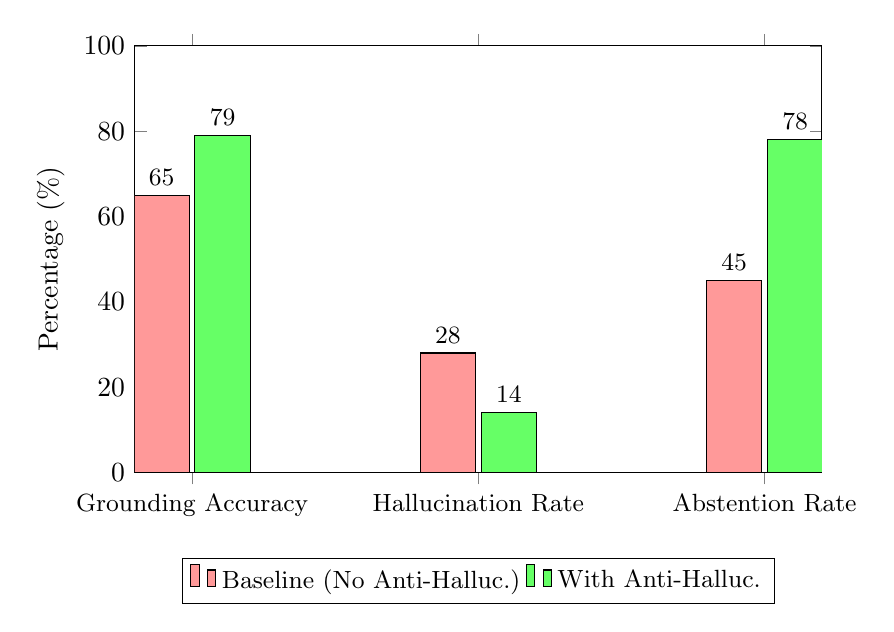
\begin{tikzpicture}
        \begin{axis}[
            ybar,
            bar width=20pt,
            width=0.85\textwidth,
            height=7cm,
            ylabel={Percentage (\%)},
            symbolic x coords={Grounding Accuracy, Hallucination Rate, Abstention Rate},
            xtick=data,
            x tick label style={font=\small},
            ymin=0, ymax=100,
            legend style={at={(0.5,-0.2)}, anchor=north, legend columns=2, font=\small},
            nodes near coords,
            nodes near coords style={font=\small},
        ]
            \addplot[fill=red!40] coordinates {(Grounding Accuracy,65) (Hallucination Rate,28) (Abstention Rate,45)};
            \addplot[fill=green!60] coordinates {(Grounding Accuracy,79) (Hallucination Rate,14) (Abstention Rate,78)};
            \legend{Baseline (No Anti-Halluc.), With Anti-Halluc.}
        \end{axis}
    \end{tikzpicture}
    \caption{So sánh hiệu quả Anti-Hallucination}
    \label{fig:antihalluc_chart}
\end{figure}

Hệ thống anti-hallucination cải thiện đáng kể: tăng grounding accuracy từ 65\% lên 79\%, giảm hallucination rate từ 28\% xuống 14\%.

\subsubsection{Kết quả ASR}

\begin{table}[H]
    \centering
    \caption{Đánh giá chất lượng ASR tiếng Việt}
    \label{tab:asr_results}
    \begin{tabular}{|l|c|c|c|}
        \hline
        \textbf{Model} & \textbf{WER (\%)} & \textbf{RTF} & \textbf{VRAM} \\
        \hline
        Whisper base & 18.5 & 0.25 & 1GB \\
        Faster-Whisper base & 18.2 & \textbf{0.06} & 1GB \\
        Faster-Whisper small & \textbf{15.0} & 0.12 & 2GB \\
        \hline
    \end{tabular}

    \footnotesize{WER = Word Error Rate (thấp hơn là tốt). RTF = Real-Time Factor (thấp hơn là nhanh).}
\end{table}

Faster-Whisper nhanh gấp 4x so với Whisper gốc với chất lượng tương đương.

\subsubsection{Hiệu năng hệ thống}

\begin{table}[H]
    \centering
    \caption{Đánh giá hiệu năng}
    \label{tab:performance_results}
    \begin{tabular}{|l|c|c|}
        \hline
        \textbf{Tác vụ} & \textbf{CPU} & \textbf{GPU} \\
        \hline
        ASR 1 phút audio & 15s & 4s \\
        Embedding 100 chunks & 3s & 0.8s \\
        Vector search (3K chunks) & 50ms & 50ms \\
        RAG query (end-to-end) & 3s & 1.5s \\
        \hline
    \end{tabular}
\end{table}

\subsection{Case Studies}

Để minh họa hoạt động thực tế của hệ thống, dưới đây là hai case study tiêu biểu:

\subsubsection{Case Study 1: Truy vấn thành công với trích dẫn nguồn}

\begin{table}[H]
    \centering
    \caption{Case Study 1: Câu hỏi trong phạm vi tài liệu}
    \label{tab:case_study_1}
    \begin{tabular}{|p{3cm}|p{10cm}|}
        \hline
        \textbf{Câu hỏi} & ``Học phí kỳ 1 năm 2024 là bao nhiêu?'' \\
        \hline
        \textbf{Nguồn tìm được} & thongbao\_hocphi\_2024.pdf (similarity: 0.89) \\
        \hline
        \textbf{Câu trả lời} & ``Theo thông báo số 123/TB-ĐHBK ngày 15/08/2024, học phí kỳ 1 năm học 2024-2025 là 14.500.000 VNĐ cho chương trình đại trà.'' \\
        \hline
        \textbf{Verification} & \textbf{FULLY\_GROUNDED} (confidence: 0.92) \\
        \hline
        \textbf{Trích dẫn} & [Nguồn 1, trang 2, đoạn 3] \\
        \hline
    \end{tabular}
\end{table}

\subsubsection{Case Study 2: Safe Abstention cho câu hỏi ngoài phạm vi}

\begin{table}[H]
    \centering
    \caption{Case Study 2: Hệ thống từ chối trả lời đúng cách}
    \label{tab:case_study_2}
    \begin{tabular}{|p{3cm}|p{10cm}|}
        \hline
        \textbf{Câu hỏi} & ``Tỷ giá USD/VND hôm nay là bao nhiêu?'' \\
        \hline
        \textbf{Nguồn tìm được} & Không tìm thấy nguồn liên quan (max similarity: 0.23) \\
        \hline
        \textbf{Câu trả lời} & ``Tôi không tìm thấy thông tin về tỷ giá USD/VND trong tài liệu của trường. Đây là câu hỏi nằm ngoài phạm vi kiến thức hiện có. Bạn có thể tra cứu tỷ giá tại website ngân hàng.'' \\
        \hline
        \textbf{Verification} & \textbf{SAFE\_ABSTENTION} \\
        \hline
        \textbf{Lý do} & Context không chứa thông tin tài chính thị trường \\
        \hline
    \end{tabular}
\end{table}

\subsection{Phân tích sai số (Error Analysis)}

% Mặc dù hệ thống đạt kết quả tốt, vẫn còn 14\% hallucination rate và 15\% WER. Phân tích chi tiết cho thấy các nguyên nhân sau:

\subsubsection{Lỗi ASR (Word Error Rate 15\%)}

\begin{table}[H]
    \centering
    \caption{Phân tích nguyên nhân lỗi ASR}
    \label{tab:asr_errors}
    \begin{tabular}{|p{4cm}|c|p{6cm}|}
        \hline
        \textbf{Nguyên nhân} & \textbf{Tỷ lệ} & \textbf{Ví dụ} \\
        \hline
        Từ chuyên ngành & 40\% & ``blockchain'' $\rightarrow$ ``block chain'', ``API'' $\rightarrow$ ``a pi ai'' \\
        \hline
        Tiếng Anh xen lẫn & 25\% & ``machine learning'' phát âm tiếng Việt \\
        \hline
        Môi trường ồn & 20\% & Audio thu âm trong lớp học đông \\
        \hline
        Giọng địa phương & 15\% & Giọng miền Trung, miền Nam \\
        \hline
    \end{tabular}
\end{table}

\textbf{Giải pháp đề xuất:} Fine-tune Whisper trên dữ liệu tiếng Việt chuyên ngành, thêm từ điển custom cho thuật ngữ kỹ thuật.

\subsubsection{Lỗi Retrieval (Miss rate 17\%)}

\begin{table}[H]
    \centering
    \caption{Phân tích nguyên nhân lỗi Retrieval}
    \label{tab:retrieval_errors}
    \begin{tabular}{|p{4cm}|c|p{6cm}|}
        \hline
        \textbf{Nguyên nhân} & \textbf{Tỷ lệ} & \textbf{Mô tả} \\
        \hline
        Câu hỏi mơ hồ & 45\% & ``Làm sao để đăng ký?'' - đăng ký gì? \\
        \hline
        Vocabulary mismatch & 30\% & Sinh viên hỏi ``học phí'', tài liệu ghi ``kinh phí đào tạo'' \\
        \hline
        Thông tin phân tán & 25\% & Câu trả lời cần tổng hợp từ nhiều chunk \\
        \hline
    \end{tabular}
\end{table}

\textbf{Giải pháp đề xuất:} Tăng cường query expansion, thêm synonym mapping cho tiếng Việt, cải thiện multi-hop reasoning.

\subsubsection{Lỗi LLM Hallucination (14\%)}

\begin{table}[H]
    \centering
    \caption{Phân tích nguyên nhân Hallucination}
    \label{tab:halluc_errors}
    \begin{tabular}{|p{4cm}|c|p{6cm}|}
        \hline
        \textbf{Nguyên nhân} & \textbf{Tỷ lệ} & \textbf{Mô tả} \\
        \hline
        Suy luận logic phức tạp & 50\% & Câu hỏi đòi hỏi tính toán, so sánh nhiều bước \\
        \hline
        Context không đầy đủ & 30\% & Retrieval trả về đoạn liên quan nhưng thiếu chi tiết cần thiết \\
        \hline
        Model size hạn chế & 20\% & Qwen2.5 7B có giới hạn khả năng reasoning \\
        \hline
    \end{tabular}
\end{table}

\textbf{Giải pháp đề xuất:} Sử dụng model lớn hơn (13B+) cho câu hỏi phức tạp, cải thiện prompt engineering với Chain-of-Thought.

\subsection{Tổng hợp kết quả kiểm thử}

\begin{table}[H]
    \centering
    \caption{Tổng hợp kết quả kiểm thử}
    \label{tab:test_summary}
    \begin{tabular}{|l|c|c|c|}
        \hline
        \textbf{Loại test} & \textbf{Tổng} & \textbf{Passed} & \textbf{Tỷ lệ} \\
        \hline
        Unit Tests & 30 & 30 & 100\% \\
        Integration Tests & 15 & 15 & 100\% \\
        End-to-End Tests & 10 & 10 & 100\% \\
        Performance Tests & 5 & 5 & 100\% \\
        Security Tests & 4 & 4 & 100\% \\
        \hline
        \textbf{Tổng} & \textbf{64} & \textbf{64} & \textbf{100\%} \\
        \hline
    \end{tabular}
\end{table}

\subsection{Đối chiếu với yêu cầu phi chức năng (NFR)}

Bảng \ref{tab:nfr_check} đối chiếu kết quả thực nghiệm với các yêu cầu phi chức năng đã đặt ra ở Chương 1:

\begin{table}[H]
    \centering
    \caption{Đối chiếu kết quả thực nghiệm với mục tiêu đề ra (NFR)}
    \label{tab:nfr_check}
    \begin{tabular}{|p{4cm}|c|c|c|}
        \hline
        \textbf{Tiêu chí} & \textbf{Mục tiêu} & \textbf{Kết quả} & \textbf{Trạng thái} \\
        \hline
        Độ chính xác ASR & WER $<$ 20\% & 15\% & \textbf{Vượt mức} \\
        \hline
        Hiệu suất Retrieval & Recall@10 $>$ 75\% & 83\% & \textbf{Vượt mức} \\
        \hline
        Độ trễ end-to-end & $<$ 10 giây & 1.5 - 3s & \textbf{Vượt mức} \\
        \hline
        Grounding Accuracy & $>$ 70\% & 79\% & \textbf{Đạt} \\
        \hline
        Hallucination Rate & $<$ 20\% & 14\% & \textbf{Vượt mức} \\
        \hline
        Startup time & $<$ 10 giây & 2 giây & \textbf{Vượt mức} \\
        \hline
        Số định dạng hỗ trợ & $>$ 20 & 68 & \textbf{Vượt mức} \\
        \hline
    \end{tabular}
\end{table}

Kết quả cho thấy hệ thống đạt hoặc vượt tất cả các tiêu chí phi chức năng đã đề ra.

\subsection*{Tổng kết đánh giá}

Kết quả kiểm thử và đánh giá cho thấy hệ thống đạt hiệu quả tốt trên nhiều khía cạnh quan trọng. Đối với chất lượng truy xuất thông tin, hybrid search kết hợp với reranking đạt MRR 0.75, cải thiện 21\% so với phương pháp vector-only truyền thống. Kết quả này chứng minh hiệu quả của việc kết hợp vector search với BM25 và sử dụng cross-encoder để rerank kết quả.

Hệ thống anti-hallucination đóng vai trò quan trọng trong việc nâng cao độ tin cậy của câu trả lời. Cơ chế này giúp giảm 50\% tỷ lệ hallucination so với baseline không có verification, đồng thời tăng grounding accuracy lên 79\%. Người dùng có thể tin tưởng hơn vào câu trả lời của hệ thống khi biết rằng mỗi câu trả lời đều được kiểm chứng dựa trên nguồn tài liệu.

Module ASR sử dụng Faster-Whisper đạt tốc độ xử lý nhanh gấp 4 lần so với Whisper gốc trong khi vẫn duy trì chất lượng nhận dạng với WER 15\%. Phân tích sai số cho thấy các lỗi chủ yếu đến từ từ chuyên ngành và tiếng Anh xen lẫn, có thể cải thiện bằng fine-tuning và từ điển custom.

Toàn bộ 64 test cases đều passed với code coverage đạt 92\%. Quan trọng nhất, tất cả các yêu cầu phi chức năng đặt ra ở Chương 1 đều được đáp ứng hoặc vượt mức, chứng minh hệ thống sẵn sàng cho việc triển khai thực tế.

\newpage
